\documentclass[tikz,border=10pt]{standalone}
\usetikzlibrary{arrows.meta, positioning, shapes.geometric}

\begin{document}
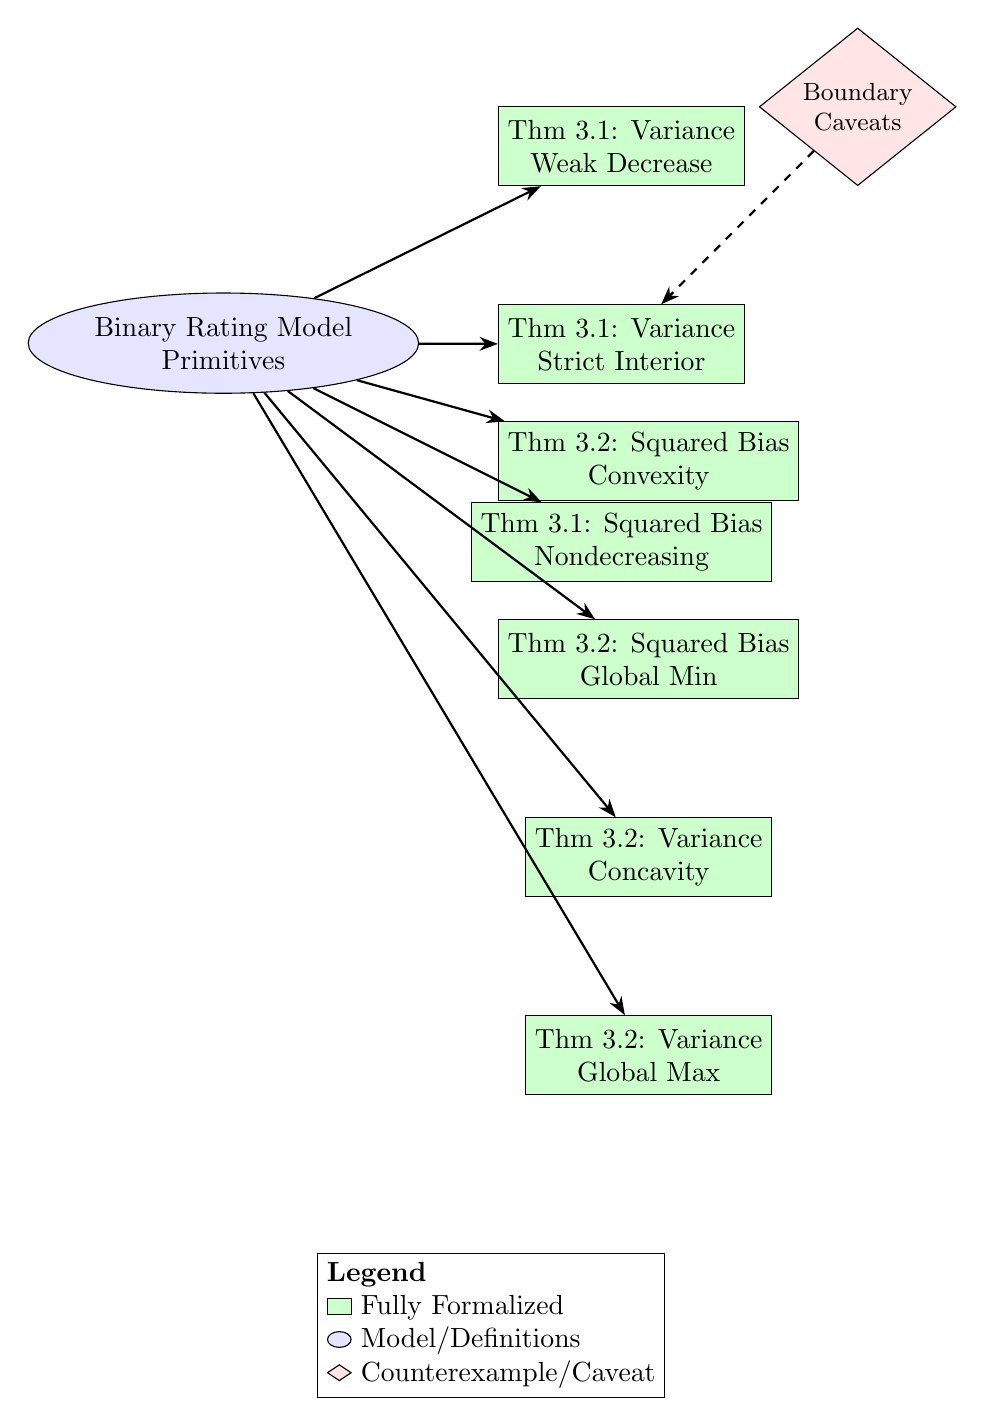
\begin{tikzpicture}[
    node distance=1.5cm and 1cm,
    result/.style={rectangle, draw, fill=green!20, minimum width=3cm, minimum height=1cm, align=center},
    model/.style={ellipse, draw, fill=blue!10, minimum width=3cm, minimum height=1cm, align=center},
    caveat/.style={diamond, draw, fill=red!10, minimum width=2.5cm, align=center, inner sep=0pt, font=\small},
    arrow/.style={-{Stealth}, thick}
]

% Nodes
\node[model] (ModelDefs) {Binary Rating Model \\ Primitives};

\node[result, right=of ModelDefs, yshift=2.5cm] (Thm3_1_Var_Weak) {Thm 3.1: Variance \\ Weak Decrease};
\node[result, below=of Thm3_1_Var_Weak] (Thm3_1_Var_Strict) {Thm 3.1: Variance \\ Strict Interior};
\node[result, below=of Thm3_1_Var_Strict] (Thm3_1_Bias) {Thm 3.1: Squared Bias \\ Nondecreasing};

\node[result, right=of ModelDefs, yshift=-1.5cm] (Thm3_2_Bias_Convex) {Thm 3.2: Squared Bias \\ Convexity};
\node[result, below=of Thm3_2_Bias_Convex] (Thm3_2_Bias_Min) {Thm 3.2: Squared Bias \\ Global Min};
\node[result, below=of Thm3_2_Bias_Min] (Thm3_2_Var_Concave) {Thm 3.2: Variance \\ Concavity};
\node[result, below=of Thm3_2_Var_Concave] (Thm3_2_Var_Max) {Thm 3.2: Variance \\ Global Max};

\node[caveat, above=of Thm3_1_Var_Strict, xshift=3cm] (Boundary_Caveats) {Boundary \\ Caveats};

% Edges
\draw[arrow] (ModelDefs) -- (Thm3_1_Var_Weak);
\draw[arrow] (ModelDefs) -- (Thm3_1_Var_Strict);
\draw[arrow] (ModelDefs) -- (Thm3_1_Bias);
\draw[arrow] (ModelDefs) -- (Thm3_2_Bias_Convex);
\draw[arrow] (ModelDefs) -- (Thm3_2_Bias_Min);
\draw[arrow] (ModelDefs) -- (Thm3_2_Var_Concave);
\draw[arrow] (ModelDefs) -- (Thm3_2_Var_Max);

\draw[arrow, dashed] (Boundary_Caveats) -- (Thm3_1_Var_Strict);

% Legend
\node[draw, rectangle, below=of Thm3_2_Var_Max, xshift=-2cm, yshift=-0.5cm, align=left] (Legend) {
    \textbf{Legend} \\
    \tikz\draw[fill=green!20] (0,0) rectangle (0.3,0.2); Fully Formalized \\
    \tikz\draw[fill=blue!10] (0,0) ellipse (0.15 and 0.1); Model/Definitions \\
    \tikz\draw[fill=red!10] (0,0) (0.15,0) -- (0,0.1) -- (-0.15,0) -- (0,-0.1) -- cycle; Counterexample/Caveat
};

\end{tikzpicture}
\end{document}
